\section{Einleitung und Versuchsziel}
\label{sec:aufgabenstellung}
%In der Aufgabenstellung wird (in eigenen Worten und ganzen Sätzen) formuliert, was das Ziel des 
%Versuches ist.  
%[Beachten Sie die eigentliche Aufgabenstellung in den Versuchsanleitungen sowie die Hinweise zur Auswertung!] 

Für eine Arbeit des \textsc{Polymerservice Merseburg (PSM)} wird ein 2L-Reaktorsystem mit automatischer Dosierung über mehrere Stunden gefordert. Weiterhin sollen über Temperaturprofile Aufheiz- und Abkühlvorgänge gesteuert werden. Beide Anforderungen sind für zwei verschiedene Polymerisationen nötig, welche an dieser Stelle nicht näher erläutert werden. 

Ziel des Projektes im Rahmen des Moduls thermischer Verfahrenstechnik II ist es, dass in Form einer studentischen Arbeit ein Prototyp für ein mögliches Reaktorsystem aufgebaut und vorgestellt wird. Die Anforderungen an das geforderte System wurden hierfür abstrahiert und vereinfacht. Dabei wird aufgezeigt welche Möglichkeiten in der Umsetzung mit bereits vorhandenen Mitteln an der \textsc{Hochschule Merseburg} bestehen.

\begin{figure}[h!]
	\centering
	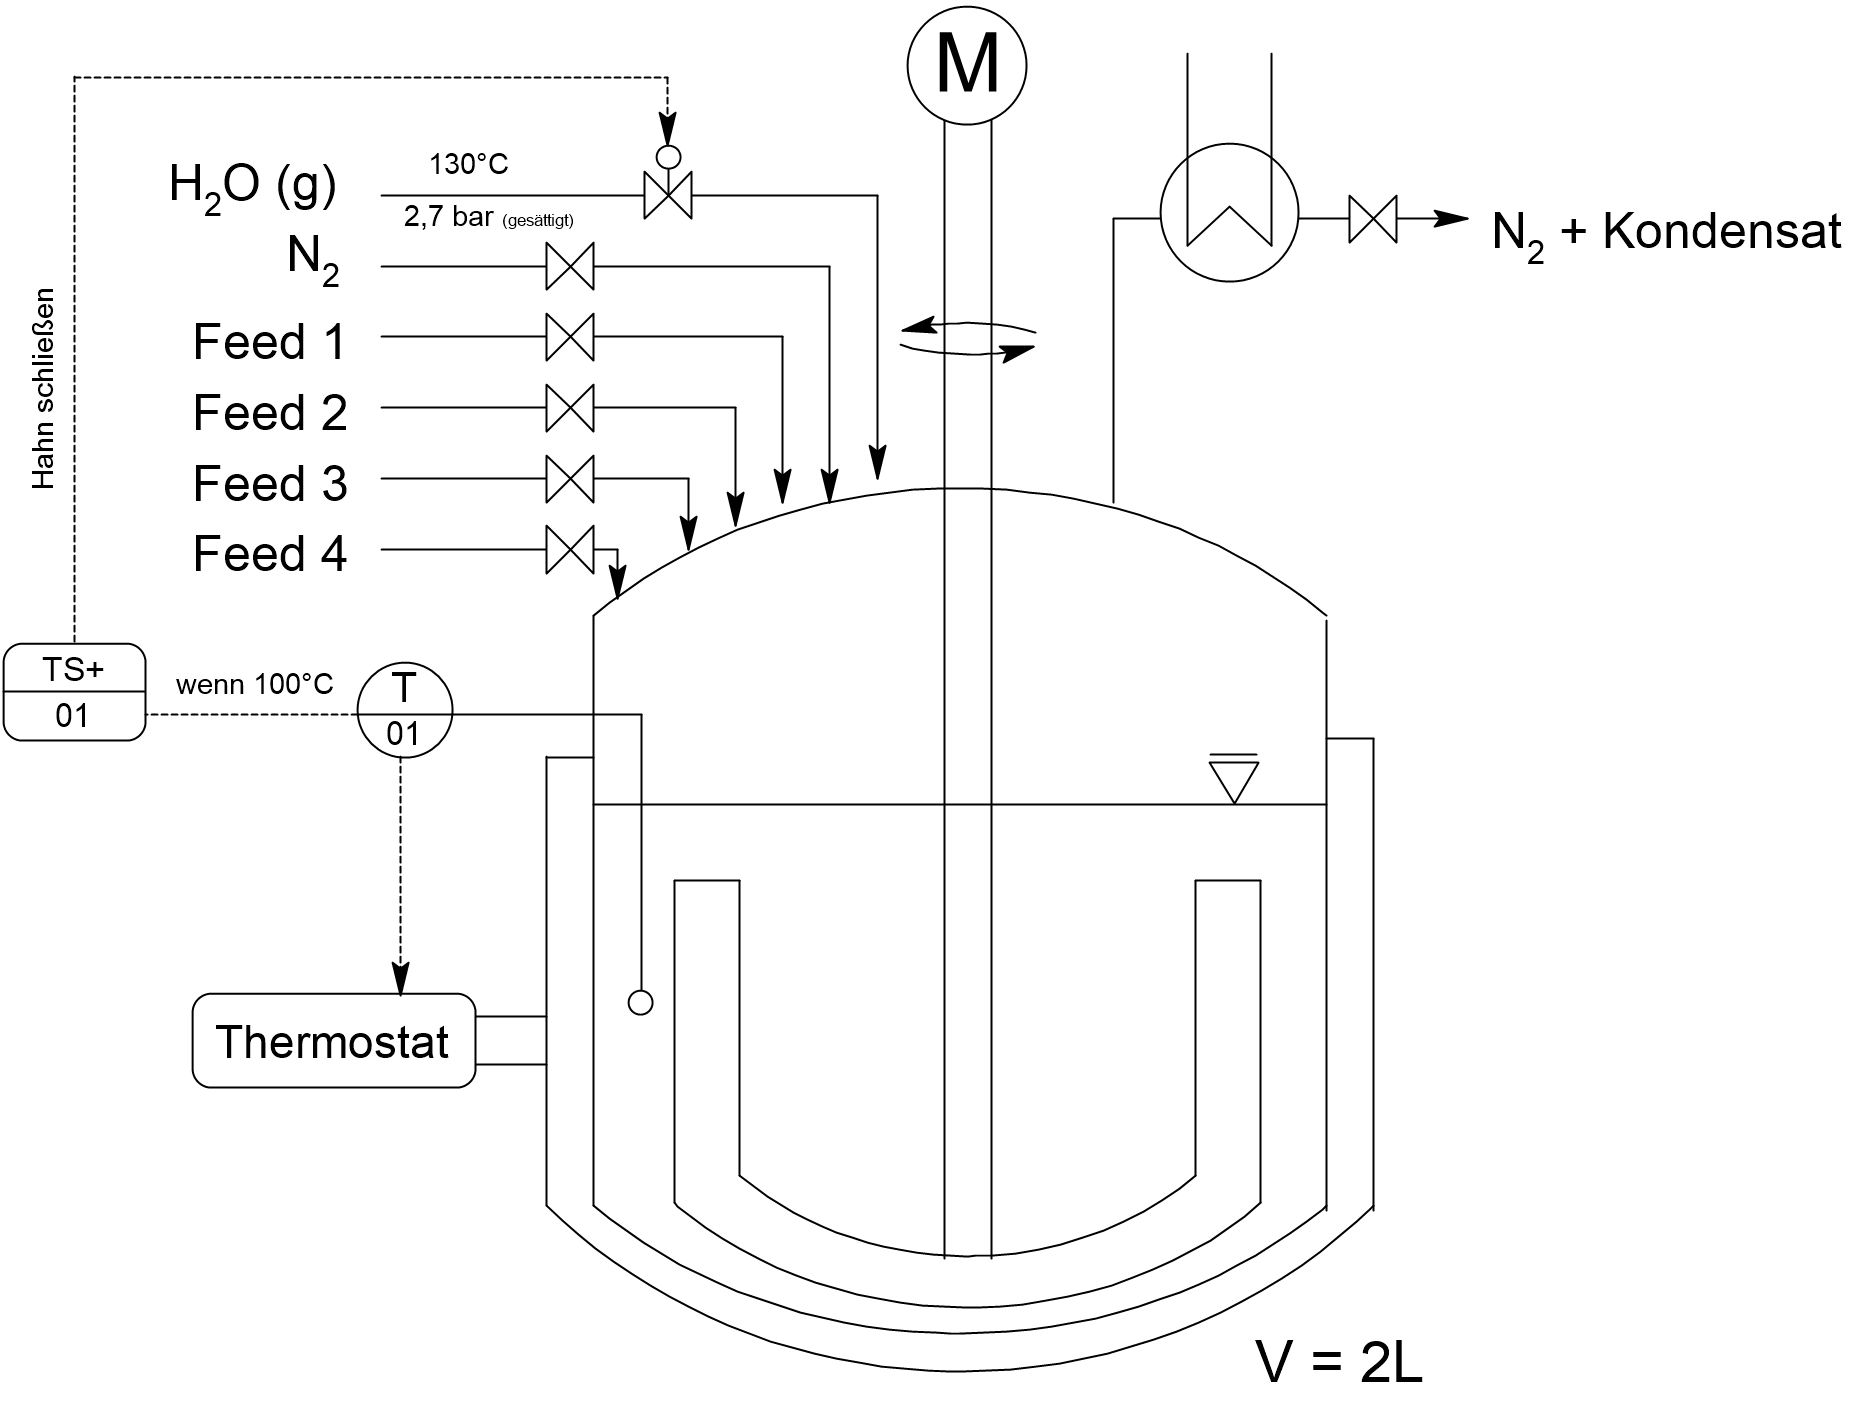
\includegraphics[width=0.75\textwidth]{img/Skizze_Prozess_1.png}
	\caption{Skizze der Anforderungen für Prozess 1}
	\label{fig:prozess 1}
\end{figure}
\FloatBarrier
%Ende